% Phase-2 progress report: baselines, pilot of all modules, errors found and fixes.
% Full-run results are NOT part of Phase 2 (they go into the final report).
% Build: .venv/bin/python scripts/phase2_report.py && cd report/phase2 && tectonic phase2_report.tex
% All numbers in generated tables and \Macros come from scripts/phase2_report.py (artifacts only).
\documentclass[conference]{IEEEtran}
\usepackage[utf8]{inputenc}
\usepackage[T1]{fontenc}
\usepackage{graphicx,booktabs,amsmath,amssymb,xcolor,tikz,hyperref,cite,array}
\usetikzlibrary{arrows.meta,positioning}
\hypersetup{colorlinks=true,linkcolor=blue!50!black,citecolor=blue!50!black,urlcolor=blue!50!black}
\graphicspath{{figures/}}
\newcommand{\BaseAcc}{43.4}
\newcommand{\BaseLo}{37.1}
\newcommand{\BaseHi}{49.9}
\newcommand{\BaseStd}{1.9}
\newcommand{\BaseTrunc}{40}
\newcommand{\BaseScSixteen}{53.7}
\newcommand{\BaseScMax}{54.7}
\newcommand{\ReproAcc}{13.8}
\newcommand{\ReproStd}{1.9}
\newcommand{\ReproLo}{10.7}
\newcommand{\ReproHi}{17.3}
\newcommand{\PilotBase}{29.5}
\newcommand{\PilotSc}{35.0}
\newcommand{\PilotPot}{41.2}
\newcommand{\PilotFull}{57.5}
\newcommand{\PilotVsSc}{+22.5}
\newcommand{\PilotVsScLo}{+7.5}
\newcommand{\PilotVsScHi}{+37.5}
\newcommand{\PilotFallback}{38}
\newcommand{\PilotCodeRan}{27}
\newcommand{\PilotKb}{56}
\newcommand{\CriticVTwoCalls}{501}
\newcommand{\CriticVTwoForced}{69}

\newcolumntype{P}[1]{>{\raggedright\arraybackslash}p{#1}}

\begin{document}
\title{Improving Scientific Reasoning in Vision-Language Models with Code Sandboxes, Agentic
Correction, Learned Verification and Retrieval on mmJEE-Eval\\[2pt]
\large Phase-2 Progress Report: Baselines, Pilot and Fixes}
\author{\IEEEauthorblockN{Arpit Kumar (12340350) \quad Saurav Gupta (12341940)}
\IEEEauthorblockA{Machine Learning course project, IIT Bhilai \quad 9 October 2026}}
\maketitle

\begin{abstract}
mmJEE-Eval shows that open vision-language models (VLMs) are weak at numerical computation and
at turning a detected error into a fix. We wrap a \emph{frozen} 4-bit VLM in an inference-time
framework with four modules: a code sandbox (program-of-thought), a Critic/Corrector loop that
localises the first wrong step, a learned solution verifier (the only trained part) and retrieval
of verified exemplars. This Phase-2 report covers the implementation, the baselines, an
end-to-end pilot and the errors we found and fixed. Our harness reproduces the base paper's
Qwen2.5-VL-7B result (\ReproAcc\% vs.\ 12.4\% on the 2025 test set), and our substrate
Qwen3-VL-8B reaches \BaseAcc\% Pass@1 with the paper's prompts. In a 40-question pilot, the full
framework reaches \PilotFull\% vs.\ \PilotBase\% for the baseline and \PilotSc\% for
compute-matched self-consistency. The pilot exposed 7 method-level problems (e.g.\ lost code
state, blocked libraries, unparsed critic replies); we explain the cause and the fix for each,
together with 11 bugs from a pre-run code review and 9 infrastructure issues.
\end{abstract}

% ----------------------------------------------------------------------------------------------
\section{Introduction and Phase-2 scope}
mmJEE-Eval~\cite{mmjee} contains 1{,}460 bilingual (English/Hindi) JEE-Advanced questions from
2019--2025, given only as images. The paper reports low accuracy for open models (12.4\% for
Qwen2.5-VL-7B on 2025) and single-pass error-correction success of only 1.1--5.2\%. It releases
an evaluation harness but no method. Our SOP proposes a training-free framework around a frozen
VLM, evaluated additively against a compute-matched self-consistency (SC)
baseline~\cite{selfconsistency}.

\textbf{This report (Phase 2)} contains:
(i) the implemented framework and evaluation harness (Sec.~\ref{sec:framework});
(ii) baselines: a reproduction of the paper with Qwen2.5-VL-7B and our substrate Qwen3-VL-8B on
the full 2025 test set (Sec.~\ref{sec:baseline});
(iii) an end-to-end pilot of all four modules on 40 test questions (Sec.~\ref{sec:pilot});
(iv) the errors found and how and why we fixed them (Sec.~\ref{sec:fixes}).
The full-scale run of all modules on all 190 test questions is the subject of the final report
(Sec.~\ref{sec:plan}).

% ----------------------------------------------------------------------------------------------
\section{Data and evaluation protocol}
\textbf{Split.} HF release \texttt{ArkaMukherjee/mmJEE-Eval}: train/dev = 2019--2024 (1{,}270
questions), test = 2025 (190 = 95 English + 95 Hindi twins; 84 Numerical, 46 MCQ-Single, 42
MCQ-Multiple, 18 Matching). The 102 questions of 2026 are excluded. Hyper-parameters, the verifier
and the RAG threshold are selected on 2024 only.

\textbf{Scoring.} \texttt{extract\_answer} and \texttt{is\_answer\_correct} are copied verbatim
from the paper's notebooks; a test checks the copies with \texttt{ast}. The public data lacks the
\texttt{acceptable\_values} column the scorer needs for range answers (e.g.\ ``8.70 TO 9.10''),
so we rebuild it on a 0.001 grid; all 691 numerical gold answers then score as correct. 12
MCQ-Single rows of 2023 with multi-letter golds are retyped MCQ-Multiple, and 4 duplicated
question IDs get unique IDs.

\textbf{Metrics.} Pass@1 = mean accuracy over samples (one ``run'' per sample index, like the
paper's run average). 95\% CIs use a cluster bootstrap over EN/HI twin pairs (2{,}000
resamples), and differences use the paired version. SC is compared at the \emph{same
generated-token budget}.

% ----------------------------------------------------------------------------------------------
\section{Framework}\label{sec:framework}
\begin{figure*}[t]
\centering
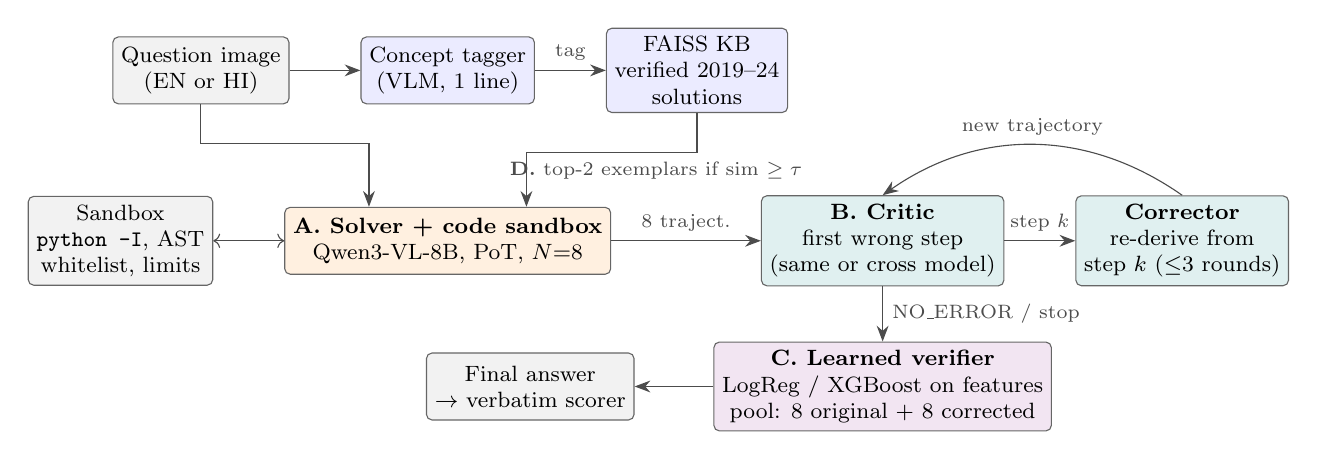
\begin{tikzpicture}[font=\footnotesize, node distance=4mm and 9mm,
  box/.style={draw=black!60, rounded corners=2pt, fill=#1, align=center, minimum height=8.5mm,
  inner sep=3pt}, box/.default=white, arr/.style={-{Stealth[length=2mm]}, black!70}]
\node[box=black!5] (img) {Question image\\(EN or HI)};
\node[box=blue!8, right=of img] (tag) {Concept tagger\\(VLM, 1 line)};
\node[box=blue!8, right=of tag] (kb) {FAISS KB\\verified 2019--24\\solutions};
\node[box=orange!12, below=13mm of tag, minimum width=34mm] (solver)
  {\textbf{A. Solver + code sandbox}\\Qwen3-VL-8B, PoT, $N{=}8$};
\node[box=black!5, left=of solver] (exec) {Sandbox\\\texttt{python -I}, AST\\whitelist, limits};
\node[box=teal!12, right=19mm of solver] (critic) {\textbf{B. Critic}\\first wrong step\\(same or cross model)};
\node[box=teal!12, right=of critic] (corr) {\textbf{Corrector}\\re-derive from\\step $k$ ($\le$3 rounds)};
\node[box=violet!10, below=7mm of critic, minimum width=40mm] (ver)
  {\textbf{C. Learned verifier}\\LogReg / XGBoost on features\\pool: 8 original + 8 corrected};
\node[box=black!5, left=10mm of ver] (out) {Final answer\\$\to$ verbatim scorer};
\draw[arr] (img) -- (tag); \draw[arr] (tag) -- node[above]{\scriptsize tag} (kb);
\draw[arr] (kb.south) -- ++(0,-5mm) -| node[pos=0.12,below]{\scriptsize \textbf{D.} top-2 exemplars if sim $\ge\tau$} ([xshift=10mm]solver.north);
\draw[arr] (img.south) -- ++(0,-5mm) -| ([xshift=-10mm]solver.north);
\draw[arr, <->] (exec) -- (solver);
\draw[arr] (solver) -- node[above]{\scriptsize 8 traject.} (critic);
\draw[arr] (critic) -- node[above]{\scriptsize step $k$} (corr);
\draw[arr] (corr.north) to[bend right=35] node[above]{\scriptsize new trajectory} (critic.north);
\draw[arr] (critic) -- node[right]{\scriptsize NO\_ERROR / stop} (ver);
\draw[arr] (ver) -- (out);
\end{tikzpicture}
\caption{Inference-time framework around a frozen VLM. Only the verifier (C) is trained, on
auto-labelled solutions of 2019--2024 questions. The KB (D) contains no 2025 question and no
near-duplicate of one.}
\label{fig:arch}
\end{figure*}

Fig.~\ref{fig:arch} shows the pipeline. The substrate is
Qwen3-VL-8B-Instruct~\cite{qwen3vl} (AWQ 4-bit), served by vLLM~\cite{vllm} on one RTX 3060
(12\,GB); InternVL3.5-8B~\cite{internvl35} (AWQ) is the cross-model critic. Sampling:
$T{=}0.7$, top-$p$ 0.8, top-$k$ 20, at most 4{,}096 new tokens per turn.

\textbf{A. Code sandbox (PoT)~\cite{pot,pal}.} The model writes ``Step $k$:'' reasoning with
\texttt{python} blocks. Generation stops at each closed block; the block runs in an isolated
subprocess (AST whitelist of math/numpy/sympy/scipy; no file or network I/O; CPU, memory and
output limits) and its output is appended before generation continues (at most 3 blocks). If no
\verb|\boxed{}| answer appears, the SOP's plain-CoT fallback is used.

\textbf{B. Agentic correction~\cite{selfrefine,critic}.} A critic receives the image and the
numbered steps and answers \texttt{FIRST\_ERROR\_STEP:~$k$} or \texttt{NO\_ERROR}. The corrector
keeps steps $1..k{-}1$ and re-derives from step $k$ (with the sandbox). The loop stops on
\texttt{NO\_ERROR}, an unchanged answer, or 3 rounds. We compare a same-model and a cross-model
critic, since self-critique alone often fails~\cite{cannotselfcorrect}.

\textbf{C. Learned verifier~\cite{cobbe,lightman}.} Training data: 8 PoT samples per training
question, labelled automatically by the verbatim scorer (pilot: 150 questions, 1{,}200
solutions). Features: length, steps, code blocks run/failed, fallback, agreement with sibling
answers, answer plausibility (format, magnitude), type/subject/language, plus a sentence
embedding. Models: logistic regression and XGBoost; GroupKFold by twin pair on 2019--2023, dev =
2024. The selected verifier picks the final answer from the 16-candidate pool.

\textbf{D. RAG~\cite{rag}.} Each question gets a one-line English concept tag (subject, topic,
method) from the VLM; tags are embedded (bge-small~\cite{bge}) and searched with
FAISS~\cite{faiss} within the same subject. The top-2 entries above a similarity threshold
$\tau$ (tuned on 2024 queries against a 2019--2023 KB) are inserted as method-only exemplars.

\textbf{Engineering.} Every model call and code execution is cached in SQLite, keyed by model,
prompt, seed and settings, so every stage resumes after a crash and evaluation runs offline.
\texttt{--pilot} runs write separately named outputs, so pilot and full results never mix.

% ----------------------------------------------------------------------------------------------
\section{Baselines}\label{sec:baseline}
\begin{table}[t]
\centering
\footnotesize
\caption{Baselines on the 2025 held-out set with the paper's prompts (single-pass CoT). Qwen2.5-VL-7B reproduces the paper's number; Qwen3-VL-8B is our substrate.}
\label{tab:baseline}
\setlength{\tabcolsep}{3.5pt}
\begin{tabular}{lrr}
\toprule
Metric (2025 test set) & Qwen2.5-VL-7B & Qwen3-VL-8B \\
\midrule
\textbf{Pass@1 (all 190)} & \textbf{13.8} & \textbf{43.4} \\
95\% CI (cluster bootstrap) & [10.7, 17.3] & [37.1, 49.9] \\
Std over runs & 1.9 (10 runs) & 1.9 (16 runs) \\
Paper (Table 3) & 12.4 $\pm$ 1.9 & -- \\
Numerical & 6.5 & 40.0 \\
MCQ-Single & 28.7 & 49.6 \\
MCQ-Multiple & 6.2 & 46.9 \\
Matching & 27.2 & 35.8 \\
English & 14.9 & 48.5 \\
Hindi & 12.6 & 38.4 \\
Mathematics & 12.0 & 55.1 \\
Chemistry & 19.5 & 41.7 \\
Physics & 9.7 & 33.2 \\
Diagram not needed & 14.0 & 48.5 \\
Diagram needed & 13.3 & 30.0 \\
Self-consistency, 16 votes & -- & 53.7 \\
Mean generated tokens / sample & -- & 2,705 \\
Samples hitting the 4{,}096 cap & -- & 40\% \\
\bottomrule
\end{tabular}
\end{table}


\textbf{Reproduction of the paper (Qwen2.5-VL-7B).} Before building on the harness we checked it
against a published number. With the paper's prompts (Appendix C), image first, and the verbatim
scorer, Qwen2.5-VL-7B scores \ReproAcc\,$\pm$\,\ReproStd\% over 10 runs (CI [\ReproLo,
\ReproHi]) vs.\ 12.4\,$\pm$\,1.9\% in the paper (Table~\ref{tab:baseline},
Fig.~\ref{fig:context}). The paper's value lies inside our CI, so prompts, image handling and
scoring match the original protocol.

\begin{figure}[t]
\centering
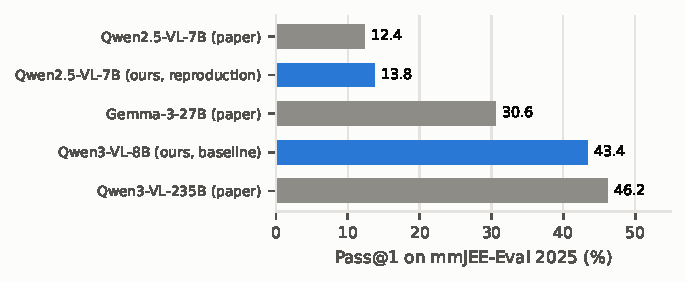
\includegraphics[width=\columnwidth]{fig_context.pdf}
\caption{Our baselines (blue) next to the base paper's numbers (grey) on 2025.}
\label{fig:context}
\end{figure}

\textbf{Substrate baseline (Qwen3-VL-8B).} Same prompts, single-pass CoT, 16 samples per question
on all 190 test questions: Pass@1 \BaseAcc\% (CI [\BaseLo, \BaseHi], run std \BaseStd). This is
far above the paper's 7B model and close to Qwen3-VL-235B (46.2\%), a model-generation effect,
since the harness reproduces the paper (above). The paper's weaknesses persist
(Fig.~\ref{fig:basebreak}): Hindi trails English by 10 points, questions that need the diagram
trail by 18 points, and Physics is the weakest subject. Majority voting over 16 samples reaches
\BaseScSixteen\% (Fig.~\ref{fig:basesc}), which is the compute-hungry reference the framework
has to beat. \BaseTrunc\% of the samples hit the 4{,}096-token cap; we keep the same cap for all
configurations. \emph{Caveat:} Qwen3-VL was released after the 2025 exam, so pre-training
exposure cannot be excluded; the paper's contamination check is part of the final report.

\begin{figure*}[t]
\centering
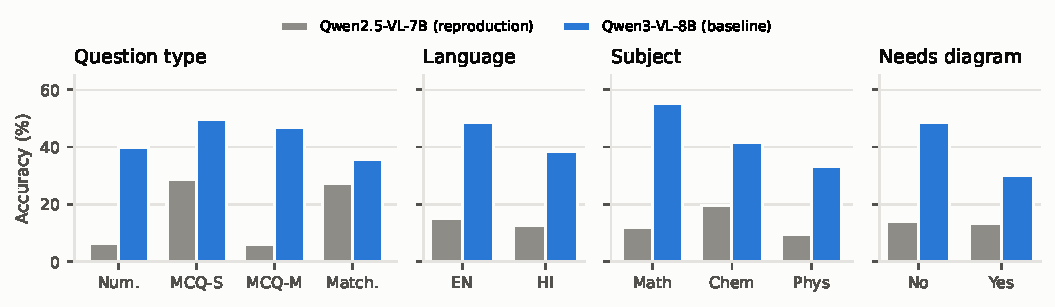
\includegraphics[width=0.95\textwidth]{fig_baseline_breakdown.pdf}
\caption{Baseline accuracy by question type, language, subject and diagram dependence.}
\label{fig:basebreak}
\end{figure*}
\begin{figure*}[t]
\centering
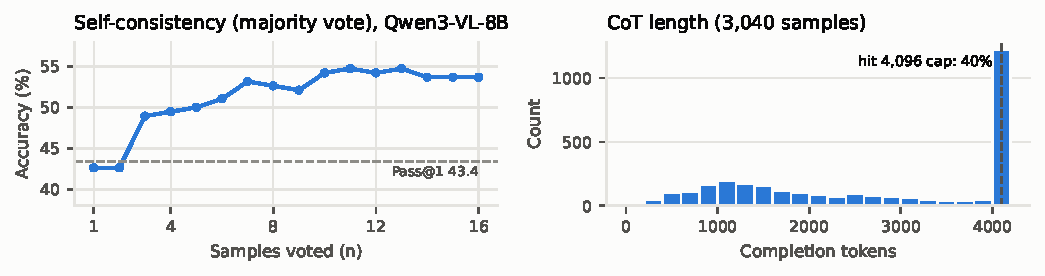
\includegraphics[width=0.95\textwidth]{fig_baseline_sc_tokens.pdf}
\caption{Qwen3-VL-8B baseline. Left: majority-vote accuracy vs.\ number of samples (dashed:
Pass@1). Right: completion length; the dashed line is the token cap.}
\label{fig:basesc}
\end{figure*}

% ----------------------------------------------------------------------------------------------
\section{Pilot of the full framework}\label{sec:pilot}
\begin{table}[t]
\centering
\footnotesize
\caption{End-to-end pilot (v1): 40 test questions (20 EN/HI pairs, stratified by type), verifier and KB from 150 training questions. Full framework vs.\ matched-compute SC: +22.5 points, paired 95\% CI [+7.5, +37.5].}
\label{tab:pilot}
\setlength{\tabcolsep}{3.5pt}
\begin{tabular}{lrcrr}
\toprule
Configuration (additive) & Acc. & 95\% CI & Num. & Tok/q \\
\midrule
Baseline (single-pass CoT) & 29.5 & [17.8, 41.6] & 19.4 & 2.7k \\
Self-consistency (matched) & 35.0 & [20.0, 52.5] & 33.3 & 43.1k \\
+ Code sandbox & 41.2 & [28.1, 54.4] & 38.9 & 3.5k \\
+ Correction (same) & 46.6 & [32.8, 60.3] & 43.1 & 7.7k \\
+ Correction (cross) & 43.1 & [29.7, 56.2] & 43.1 & 5.5k \\
+ Learned verifier & 50.0 & [32.5, 67.5] & 50.0 & 44.0k \\
+ Retrieval (RAG) & 57.5 & [40.0, 72.5] & 55.6 & 46.6k \\
\bottomrule
\end{tabular}
\end{table}


\textbf{Setup.} The pilot runs every module end-to-end on 40 test questions (20 EN/HI twin pairs,
stratified by question type) with a verifier and KB built from 150 training questions (8 PoT
samples each). It was run before the fixes of Sec.~\ref{sec:fixes} (``v1''). The pilot questions
are harder than average (baseline \PilotBase\% vs.\ \BaseAcc\% on all 190).

\textbf{Results} (Table~\ref{tab:pilot}, Figs.~\ref{fig:pilot}--\ref{fig:pilotcompute}). Each
module adds accuracy: the code sandbox lifts the baseline from \PilotBase\% to \PilotPot\%,
correction adds 2--5 points, the verifier and RAG bring the full framework to \PilotFull\%.
The full framework beats SC at the same token budget by \PilotVsSc{} points (paired CI
[\PilotVsScLo, \PilotVsScHi]). With 40 questions the CIs are about $\pm$15 points, so these
numbers are preliminary; they show that the pipeline works end to end and where it fails.

\begin{figure}[t]
\centering
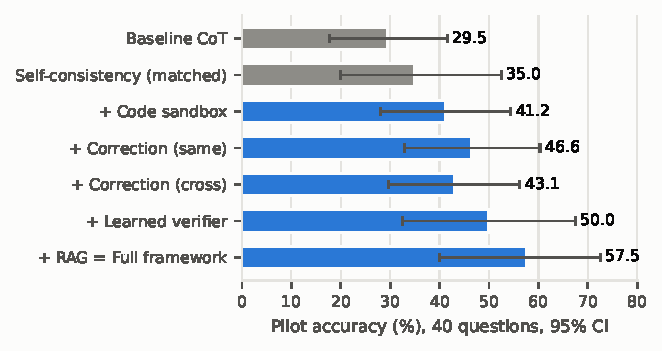
\includegraphics[width=\columnwidth]{fig_pilot.pdf}
\caption{Pilot (v1), additive rows with 95\% CIs.}
\label{fig:pilot}
\end{figure}
\begin{figure}[t]
\centering
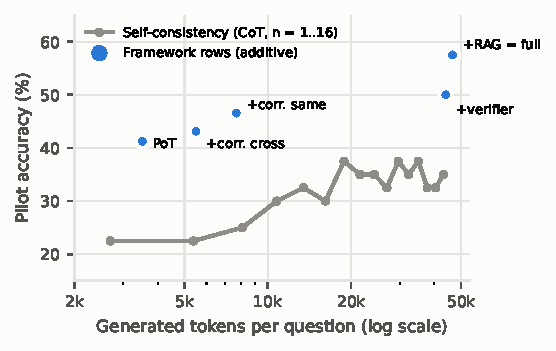
\includegraphics[width=\columnwidth]{fig_pilot_compute.pdf}
\caption{Pilot accuracy vs.\ generated tokens per question. Grey: SC over $n$ CoT samples. The
framework rows lie above the SC curve at every budget.}
\label{fig:pilotcompute}
\end{figure}

\begin{table*}[t]
\centering
\footnotesize
\caption{Correction loop in the pilot (v1, 320 chains each). Detect = critic flags an originally wrong solution; False al. = flags a correct one; Fix$|$det. = detected wrong solutions that end correct.}
\label{tab:corr}
\setlength{\tabcolsep}{3.5pt}
\begin{tabular}{lrrrrrr}
\toprule
Critic & Before $\to$ after & Detect & False al. & Fix$|$det. & W$\to$R / R$\to$W & Unparsed \\
\midrule
Same-model (Qwen3-VL) & 41.2 $\to$ 46.6 & 79.3 & 53.0 & 16.8 & 25 / 8 & 0 \\
Cross-model (InternVL3.5) & 41.2 $\to$ 43.1 & 35.1 & 23.5 & 19.7 & 13 / 7 & 76 \\
Full (RAG, cross) & 42.8 $\to$ 46.2 & 40.4 & 21.2 & 20.3 & 15 / 4 & 76 \\
Base paper (single pass) &  &  &  & 1.1--5.2 &  &  \\
\bottomrule
\end{tabular}
\end{table*}

\begin{figure*}[t]
\centering
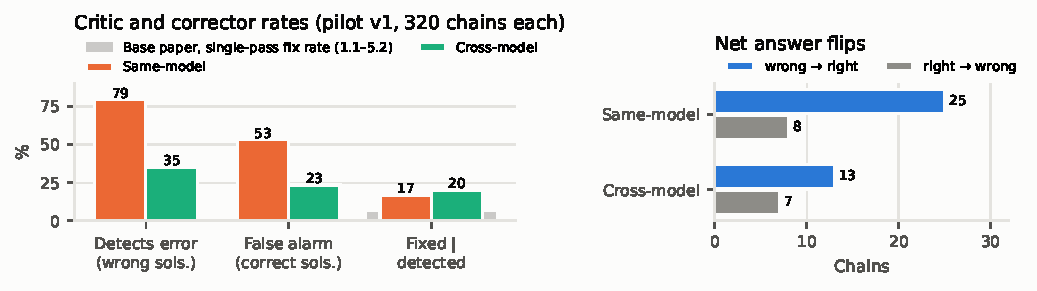
\includegraphics[width=0.92\textwidth]{fig_pilot_correction.pdf}
\caption{Correction loop in the pilot (v1). Left: detection, false alarms and the fraction of
detected wrong solutions that end correct (grey band: the base paper's single-pass 1.1--5.2\%).
Right: answers flipped wrong$\to$right vs.\ right$\to$wrong.}
\label{fig:pilotcorr}
\end{figure*}

\textbf{Correction} (Table~\ref{tab:corr}, Fig.~\ref{fig:pilotcorr}). The step-localised,
multi-round loop fixes 17--20\% of the wrong solutions its critic detects, well above the
paper's single-pass 1.1--5.2\%. The same-model critic flags almost everything (79\% detection
but 53\% false alarms); the cross-model critic was hampered by unparsed replies (76), which
motivated fix~3 below.

\begin{figure*}[t]
\centering
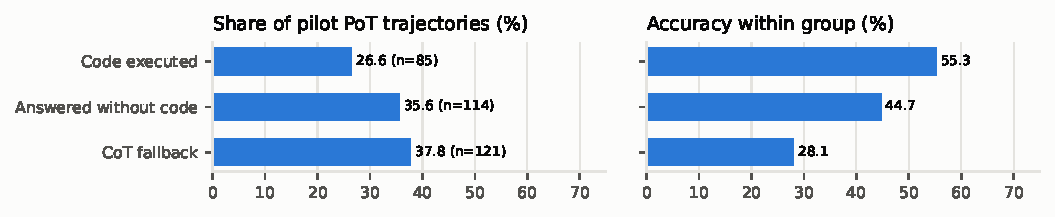
\includegraphics[width=0.92\textwidth]{fig_pilot_anatomy.pdf}
\caption{Pilot PoT trajectories (320) by outcome, and accuracy within each group.}
\label{fig:anatomy}
\end{figure*}

\textbf{How the sandbox is used} (Fig.~\ref{fig:anatomy}). Only \PilotCodeRan\% of
trajectories execute code, and they are the most accurate. \PilotFallback\% end in the CoT
fallback, with the lowest accuracy; this motivated the analysis in fix~4.

\begin{table}[t]
\centering
\footnotesize
\caption{Learned verifier in the pilot (1,200 auto-labelled solutions, 47.6\% correct). CV: GroupKFold by twin pair on 2019--2023; dev: 2024; test: the 2025 pilot pool (16 candidates per question). Test sel.\ = selection accuracy (weighted vote).}
\label{tab:verifier}
\setlength{\tabcolsep}{3.5pt}
\begin{tabular}{lrrrrr}
\toprule
Model / features & CV AUC & Dev AUC & F1 & Test AUC & Test sel. \\
\midrule
LR / handcrafted & 0.858 & 0.867 & 0.736 & 0.781 & 55.0 \\
LR / embedding & 0.704 & 0.608 & 0.619 & 0.570 & 57.5 \\
LR / all & 0.863 & 0.876 & 0.743 & 0.794 & 57.5 \\
XGB / handcrafted & 0.855 & 0.874 & 0.754 & 0.794 & 55.0 \\
XGB / embedding & 0.622 & 0.591 & 0.588 & 0.603 & 55.0 \\
XGB / all & 0.847 & 0.870 & 0.785 & 0.807 & 55.0 \\
Majority vote &  &  &  &  & 55.0 \\
Oracle (any correct) &  &  &  &  & 75.0 \\
\bottomrule
\end{tabular}
\end{table}

\begin{figure}[t]
\centering
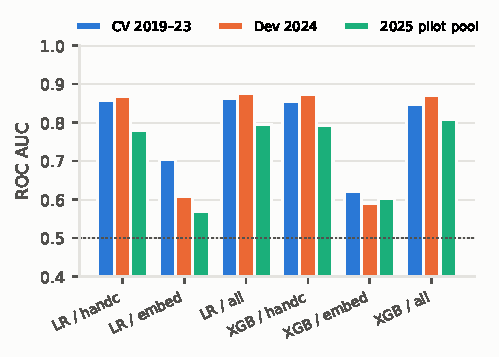
\includegraphics[width=\columnwidth]{fig_verifier_pilot.pdf}
\caption{Pilot verifier: ROC AUC per model and feature set (handcrafted, embedding, all).}
\label{fig:verifier}
\end{figure}

\textbf{Verifier} (Table~\ref{tab:verifier}, Fig.~\ref{fig:verifier}). Correctness is
predictable: AUC $\approx$0.87 on the 2024 dev year and 0.78--0.81 on the 2025 pilot pool with
handcrafted features, which carry most of the signal; the sentence embedding alone is weak
(0.57--0.70). With only 1{,}200 training solutions, selection is at most 2.5 points above
majority voting and far below the oracle (75\%), so the main headroom is in selection.

\textbf{RAG.} The pilot KB has only \PilotKb{} entries (only the 56 of the 75 pilot training
pairs that had a verified-correct solution), and only 4 of the 40 questions retrieved an exemplar. The pilot
therefore cannot attribute the last gain to retrieval; the final KB is built from all 1{,}270
training questions.

% ----------------------------------------------------------------------------------------------
\section{Errors found and fixes}\label{sec:fixes}
We found problems in three ways: by reading the pilot traces (1{,}520 PoT trajectories = 320
test + 1{,}200 training, and 320 correction chains per critic), by a pre-run code review with
three parallel reviewers, and while setting up the lab GPU. For each problem we report the
evidence, why it matters and what we changed. Every code fix has a regression test.

\begin{table*}[t]
\centering\scriptsize
\caption{Method-level problems found in the pilot traces: evidence, reason for fixing, and fix.}
\label{tab:pilotfixes}
\setlength{\tabcolsep}{3pt}
\begin{tabular}{@{}P{0.2cm}P{2.1cm}P{3.9cm}P{3.6cm}P{4.4cm}P{2.6cm}@{}}
\toprule
\# & Problem & Evidence (how we found it) & Why it matters & What we did & Effect (v2) \\
\midrule
1 & Code state lost between blocks & 47 \texttt{NameError}s: every block ran in a fresh process,
but the model reuses variables from its earlier blocks & Correct computations failed; the
solution then fell back to mental arithmetic, the weakness PoT is meant to remove & Earlier
blocks of the same solution are replayed silently (only those that pass the safety check) before
the new block & 0 \texttt{NameError}s \\
2 & Needed library blocked & 86 blocked blocks: \texttt{scipy.optimize}/\texttt{integrate}
(root finding, integrals) were not on the whitelist & The model chose the right tool and was
refused & \texttt{scipy} allowed; file-I/O and parser submodules (\texttt{scipy.io},
\texttt{sympy.parsing}) stay blocked & 0 blocked \\
3 & Critic gives no verdict & 76 InternVL replies unparsed; 75 of them hit the 1{,}536-token
cap because the critic re-solved the whole problem & No verdict $\Rightarrow$ no correction, so
the cross-model critic looked weak for a formatting reason & Prompt asks for a short check;
\emph{verdict forcing}: a cut-off reply gets a short greedy continuation after a decision cue &
1/\CriticVTwoCalls{} unparsed (\CriticVTwoForced{} forced); detection 35$\to$56\% \\
4 & Many CoT fallbacks & Fallback in 35--42\% of PoT runs; 480 of 539 were the model reasoning
without code until the token cap (``Wait, perhaps\ldots'' loops); only 9 were code failures &
Fallback answers are the least accurate and cost a second generation & A/B test on the 480: force
an answer from the truncated text vs.\ the SOP fallback: 21.9\% vs.\ 30.0\% & Forcing
\emph{rejected}; SOP fallback kept (negative result) \\
5 & SC baseline under-sampled & The full framework used as many tokens as 18 CoT samples, but
only 16 existed & A too-weak SC baseline would overstate our gain & CoT raised to 20 samples per
question for the final run & Fair matched compute \\
6 & Verifier $\approx$ majority vote & Dev selection 54.2\% = majority vote, despite AUC 0.87 &
Selection is the verifier's job; claiming a gain would be wrong & Reported honestly
(\texttt{primary\_beats\_majority\_on\_dev} flag); final verifier trains on $\approx$8$\times$ more
data & Open; re-tested at scale \\
7 & One prompt aborted a batch & In the v2 run a long multi-round solution gave a 12{,}303-token
critic prompt ($>$12{,}288 context); vLLM's \texttt{VLLMValidationError} is not a
\texttt{ValueError}, so the whole batch aborted & One bad request could kill hours of batched
GPU work & Validation errors are caught, the batch is retried request by request, and only the
bad request returns an empty (conservatively handled) result & No batch aborts since \\
\bottomrule
\end{tabular}
\end{table*}

\textbf{Fixes from the pilot} (Table~\ref{tab:pilotfixes}). We re-ran PoT and the cross-model
correction on the same 40 questions with the fixes (``v2'', Table~\ref{tab:fixes},
Fig.~\ref{fig:fixes}). The engineering failures are gone: no blocked or crashed code, and the
critic returns a verdict for 500 of 501 calls. The critic now \emph{detects} many more errors
(56\% vs.\ 35\%), but its net effect on accuracy is unchanged within noise; turning detections
into fixes remains the bottleneck, as in the paper. Fig.~\ref{fig:forcing} shows the A/B test
behind fix~4: forcing an answer from truncated reasoning is worse on three of four question
types, so we kept the SOP's fallback.

\begin{table}[t]
\centering
\footnotesize
\caption{Verification run of the fixes on the same pilot questions.}
\label{tab:fixes}
\setlength{\tabcolsep}{3.5pt}
\begin{tabular}{lrr}
\toprule
Pilot check (40 q, cross critic) & v1 & v2 \\
\midrule
Code blocks executed OK & 119 & 138 \\
Blocked by sandbox whitelist & 13 & 0 \\
NameError (state lost) & 3 & 0 \\
PoT accuracy (320 traj.) & 41.2 & 41.2 \\
Critic calls / unparsed & 431 / 76 & 501 / 1 \\
Verdicts via verdict forcing & -- & 69 \\
Critic detection rate & 35.1 & 56.4 \\
Critic false-alarm rate & 23.5 & 29.5 \\
Acc.\ before $\to$ after & 41.2 $\to$ 43.1 & 41.2 $\to$ 41.9 \\
\bottomrule
\end{tabular}
\end{table}

\begin{figure}[t]
\centering
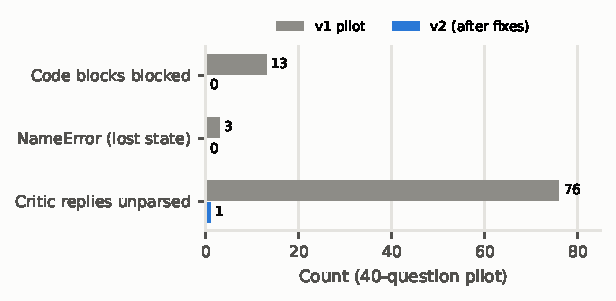
\includegraphics[width=\columnwidth]{fig_fixes.pdf}
\caption{Failures in the pilot before (v1) and after (v2) the fixes.}
\label{fig:fixes}
\end{figure}
\begin{figure}[t]
\centering
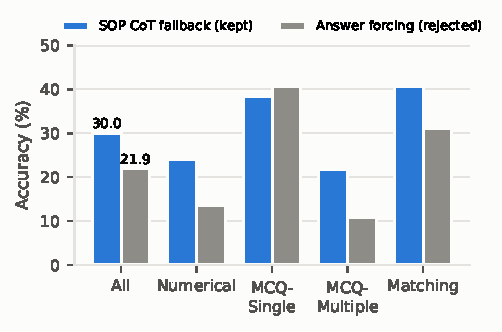
\includegraphics[width=\columnwidth]{fig_forcing_ab.pdf}
\caption{A/B test of fix~4 on the 480 pilot trajectories that hit the token cap: accuracy of the
SOP CoT fallback vs.\ forcing an answer from the truncated reasoning.}
\label{fig:forcing}
\end{figure}

\begin{table*}[t]
\centering\scriptsize
\caption{Bugs found by the pre-run code review (three parallel reviewers), all fixed before any
GPU run.}
\label{tab:review}
\setlength{\tabcolsep}{3pt}
\begin{tabular}{@{}P{0.3cm}P{4.3cm}P{5.1cm}P{6.8cm}@{}}
\toprule
\# & Problem & Why it matters & What we did \\
\midrule
8 & Verifier cross-validation crashed: \texttt{GroupKFold} returns positions, pandas read them as
labels & No verifier could be trained & Positional indexing (\texttt{iloc}) \\
9 & Verifier features differed between training (pool of 8) and test (pool of 16; cumulative
token counts) & Train/test mismatch silently degrades the verifier & Features computed per
sub-pool; each solution stores its own token count \\
10 & Sandbox read unbounded stdout into the parent (reproduced: 8\,GB RAM) & A printing loop could
crash the 15\,GB lab PC & Output written to files capped by \texttt{RLIMIT\_FSIZE} \\
11 & Model ending its turn right after a code fence: code never ran & Silent loss of tool use &
Detected; the block is executed and generation continues \\
12 & No context-length guard & Long multi-turn prompts fail & Per-turn token budget and
per-request retry \\
13 & Critic-explanation regex took the first match, not the last & Wrong step passed to the
corrector & Last match used \\
14 & \texttt{--config} not passed to the subprocesses of cross-model phases & Phases could run
with different settings & Passed through \\
15 & CIs ignored the EN/HI twin correlation & Over-confident intervals (twins are near-duplicate
questions) & Cluster bootstrap over twin pairs \\
16 & Range grid of 0.01 rejected valid in-range answers (e.g.\ 0.275) & Correct answers scored
wrong & 0.001 grid; test: all 691 golds score correct \\
17 & Duplicate question IDs could merge two questions in the KB & Wrong exemplars, possible
leakage & Unique twin keys \\
18 & Mock VLM ignored the image, which hid bug 8 & Tests passed while the pipeline was broken &
Image-dependent mock; end-to-end mock test now passes \\
\bottomrule
\end{tabular}
\end{table*}

\begin{table*}[t]
\centering\scriptsize
\caption{Infrastructure issues on the lab GPU (RTX 3060 12\,GB, 15\,GB RAM, shared PC).}
\label{tab:infra}
\setlength{\tabcolsep}{3pt}
\begin{tabular}{@{}P{0.3cm}P{5.3cm}P{4.6cm}P{6.3cm}@{}}
\toprule
\# & Problem (evidence) & Why it matters & What we did \\
\midrule
19 & vLLM KV cache did not fit (0.36\,GiB free after weights) & Model would not start or ran at
batch size 1 & Capped image pixels, \texttt{max\_num\_batched\_tokens}=4096, FP8 KV cache:
1.9$\times$ throughput (measured) \\
20 & flashinfer JIT compile failed (no \texttt{ninja}) & Engine crash at start & PyTorch sampler
\\
21 & rsync exclude pattern also skipped \texttt{src/.../report} & Lab code incomplete & Anchored
exclude patterns \\
22 & CUDA out of memory during transcription at 0.92 memory utilisation & Stage crash & 0.88
utilisation, 32 concurrent sequences \\
23 & vLLM's InternVL processor rejects \texttt{max\_dynamic\_patch} & Critic could not load &
Default tiling \\
24 & FP8 KV cache produced garbage with Qwen2.5-VL (1.8\% accuracy, junk tokens) & Reproduction
would be invalid & Normal KV cache for that model; its cached outputs invalidated \\
25 & PoT prompt produced too little code & Sandbox rarely used & Format example and a
conciseness rule in the prompt \\
26 & systemd-oomd killed the whole tmux session under memory pressure (10.5\,h lost) & Silent
loss of long runs & Each stage in its own scope with 3 retries; sandbox workers 8$\to$4 \\
27 & oomd also kills \texttt{systemd-run --user} scopes (it watches all of the user service) &
Same as 26 & Jobs started with \texttt{nohup}+\texttt{setsid} from the ssh session, outside that
policy; supervisor with retries plus a quiet local watcher \\
\bottomrule
\end{tabular}
\end{table*}

\textbf{Code review and infrastructure} (Tables~\ref{tab:review}--\ref{tab:infra}). Before
spending GPU time, three reviewers checked data/scoring/metrics, sandbox/PoT/agents and
verifier/RAG/leakage in parallel and found 11 bugs; the most serious would have crashed the
verifier (8), mismatched its train and test features (9) or made intervals too narrow (15).
The lab issues were mostly memory limits of the 12\,GB GPU and the shared PC's out-of-memory
daemon.

\textbf{Testing.} 73 \texttt{pytest} tests run on CPU with a mock VLM: scorer identity with the
notebooks and all gold answers, extraction cases, sandbox limits (timeout, memory, blocked
imports, output cap, replay, scipy), PoT and correction loops (fallback, verdict forcing, stop
rules), verifier on synthetic data (AUC $>$ 0.9) and CV indexing, RAG filters and threshold,
leakage assertions (no 2025 twin in any training data or KB) and an end-to-end pipeline run.

% ----------------------------------------------------------------------------------------------
\section{Plan for the final report}\label{sec:plan}
The full run applies the fixed (v2) pipeline to all 190 test questions and all 1{,}270 training
questions on the lab GPU: CoT with 20 samples; PoT with 8 samples; same- and cross-model
correction; PoT on the training set (verifier data and KB); RAG-PoT; full-framework correction;
verifier training and best-of-16 selection; and the paper's contamination check. The final
report will contain the complete SOP Table~I with matched-compute SC, significance tests,
per-type/language/subject breakdowns, correction statistics compared with the paper, and the
discussion.

\section{Limitations}
One substrate model and one test year (190 questions); the pilot has only 40 questions (CIs
about $\pm$15 points); 4-bit weights and a 4{,}096-token budget (\BaseTrunc\% of baseline samples
are truncated); the strict, unchanged scorer (no partial credit, first \verb|\boxed{}| only);
possible pre-training exposure of Qwen3-VL to the 2025 exam.

\clearpage
\begin{thebibliography}{99}\footnotesize
\bibitem{mmjee} A.~Mukherjee and S.~Ghosh, ``mmJEE-Eval: A bilingual multimodal benchmark for
evaluating scientific reasoning in vision-language models,'' in \emph{Proc.\ IJCNLP-AACL}, 2025.
\bibitem{selfconsistency} X.~Wang \emph{et al.}, ``Self-consistency improves chain of thought
reasoning in language models,'' in \emph{Proc.\ ICLR}, 2023.
\bibitem{pot} W.~Chen \emph{et al.}, ``Program of thoughts prompting: Disentangling computation
from reasoning for numerical reasoning tasks,'' \emph{TMLR}, 2023.
\bibitem{pal} L.~Gao \emph{et al.}, ``PAL: Program-aided language models,'' in \emph{Proc.\
ICML}, 2023.
\bibitem{selfrefine} A.~Madaan \emph{et al.}, ``Self-Refine: Iterative refinement with
self-feedback,'' in \emph{Proc.\ NeurIPS}, 2023.
\bibitem{critic} Z.~Gou \emph{et al.}, ``CRITIC: Large language models can self-correct with
tool-interactive critiquing,'' in \emph{Proc.\ ICLR}, 2024.
\bibitem{cannotselfcorrect} J.~Huang \emph{et al.}, ``Large language models cannot self-correct
reasoning yet,'' in \emph{Proc.\ ICLR}, 2024.
\bibitem{cobbe} K.~Cobbe \emph{et al.}, ``Training verifiers to solve math word problems,''
arXiv:2110.14168, 2021.
\bibitem{lightman} H.~Lightman \emph{et al.}, ``Let's verify step by step,'' in \emph{Proc.\
ICLR}, 2024.
\bibitem{rag} P.~Lewis \emph{et al.}, ``Retrieval-augmented generation for knowledge-intensive
NLP tasks,'' in \emph{Proc.\ NeurIPS}, 2020.
\bibitem{faiss} J.~Johnson, M.~Douze and H.~J\'egou, ``Billion-scale similarity search with
GPUs,'' \emph{IEEE Trans.\ Big Data}, 2019.
\bibitem{bge} S.~Xiao \emph{et al.}, ``C-Pack: Packed resources for general Chinese
embeddings,'' in \emph{Proc.\ SIGIR}, 2024.
\bibitem{vllm} W.~Kwon \emph{et al.}, ``Efficient memory management for large language model
serving with PagedAttention,'' in \emph{Proc.\ SOSP}, 2023.
\bibitem{qwen3vl} Qwen Team, ``Qwen3-VL,'' model release and technical report, 2025.
\bibitem{internvl35} OpenGVLab, ``InternVL3.5,'' model release and technical report, 2025.
\end{thebibliography}
\end{document}
